\documentclass[12pt, titlepage]{article}

\usepackage{fullpage}
\usepackage[round]{natbib}
\usepackage{multirow}
\usepackage{booktabs}
\usepackage{tabularx}
\usepackage{graphicx}
\usepackage{float}
\usepackage{hyperref}
\hypersetup{
    colorlinks,
    citecolor=black,
    filecolor=black,
    linkcolor=red,
    urlcolor=blue
}
\usepackage[round]{natbib}

\newcounter{acnum}
\newcommand{\actheacnum}{AC\theacnum}
\newcommand{\acref}[1]{AC\ref{#1}}

\newcounter{ucnum}
\newcommand{\uctheucnum}{UC\theucnum}
\newcommand{\uref}[1]{UC\ref{#1}}

\newcounter{mnum}
\newcommand{\mthemnum}{M\themnum}
\newcommand{\mref}[1]{M\ref{#1}}

\title{SE 3XA3: Module Guide\\GardenDefender}

\author{Team 29
		\\ Ashley Williams, willia18
		\\ Declan Mullane, mullanem
		\\ Leo Shi, shiy12
}

\date{November 8, 2018}

%\input{../../Comments}

\begin{document}

\maketitle

\pagenumbering{roman}
\tableofcontents
\listoftables
\listoffigures

\begin{table}[bp]
\caption{\bf Revision History}
\begin{tabularx}{\textwidth}{p{3cm}p{2cm}X}
\toprule {\bf Date} & {\bf Version} & {\bf Notes}\\
\midrule
Nov. 6th, 2018 & 1.0 & Initial Draft\\
Nov. 8th, 2018 & 1.1 & Updating All Sections\\
%Date 2 & 1.1 & Notes\\
\bottomrule
\end{tabularx}
\end{table}

\newpage

\pagenumbering{arabic}

\section{Introduction}\label{SecIntro}


Garden Defender is a re-implementation of a downloadable shooter game to make it accessible via web browser. Through this re-implementation, the project aims to alleviate boredom and provide entertainment on a new platform for a wider range of people.  

This module guide document(MG) decomposes s system into modules and ensures they meet the functional and non-functional requirements specified in the software Requirements Specification document(SRS). Meanwhile, a module interface specification document(MIS) is also created to elaborate on the syntax and semantic of modules provided in the MG.

Design principles been used in Garden Defender are information hiding and making the uses relation a hierarchy. Information hiding is applied so that even when the module secret changes, the module design interface does not need to change. These principles also ensure the high cohesion within a module and low coupling between modules. 


The document is organized as follows:
\begin{itemize}
\item Section \ref{SecIntro} gives a brief overview of our project and an introduction to the module design document.
\item Section \ref{SecChange} lists anticipated and unlikely changes from Software Requirement Specification document.
\item Section \ref{SecMH} summarizes all the modules and gives an overview of the module design.
\item Section \ref{SecConnection}, along with table \ref{TblRT}, shows the connection between requirements and design.
\item Section \ref{SecMD} provides the module decomposition details including secrets, services and implemented by information for each module.
\item Section \ref{SecTM} consists of two traceability matrices. Table \ref{TblRT} shows the connection between modules and requirements. Table \ref{TblACT} connects the anticipated changes to modules.
\item Section \ref{SecUse} gives the hierarchy diagram and describes the use relation between modules.
\end{itemize}

\section{Anticipated and Unlikely Changes} \label{SecChange}

This section lists possible changes to the system. According to the likeliness
of the change, the possible changes are classified into two
categories. Anticipated changes are listed in Section \ref{SecAchange}, and
unlikely changes are listed in Section \ref{SecUchange}.

\subsection{Anticipated Changes} \label{SecAchange}

Anticipated changes are the source of the information that is to be hidden
inside the modules. Ideally, changing one of the anticipated changes will only
require changing the one module that hides the associated decision. The approach
adapted here is called design for
change.

\begin{description}
\item[\refstepcounter{acnum} \actheacnum \label{acHardware}:] The specific
  hardware on which the software is running.
\item[\refstepcounter{acnum} \actheacnum \label{acInput}:] The format of the input data for game play may change to accommodate mobile browsers as well as computer browsers.
\item[\refstepcounter{acnum} \actheacnum \label{acScreenDim}:] The game screen resolution may be adjusted to accommodate both mobile and computer browsers. 
\item[\refstepcounter{acnum} \actheacnum \label{acGraphics}:] Before final version of game, graphics will likely be modified. 
\item[\refstepcounter{acnum} \actheacnum \label{acLevel}:] Level difficulty, length, and features (different enemies and weapons) are likely to be modified. 
\item[\refstepcounter{acnum} \actheacnum \label{acUserGuide}:] The user guide is likely to be updated as levels are updated. 
\end{description}

\subsection{Unlikely Changes} \label{SecUchange}

The module design should be as general as possible. However, a general system is
more complex. Sometimes this complexity is not necessary. Fixing some design
decisions at the system architecture stage can simplify the software design. If
these decision should later need to be changed, then many parts of the design
will potentially need to be modified. Hence, it is not intended that these
decisions will be changed.

\begin{description}
\item[\refstepcounter{ucnum} \uctheucnum \label{ucIO}:] Input (game file, keyboard) and Output (game file, screen, speakers) devices. 
\item[\refstepcounter{ucnum} \uctheucnum \label{ucInput}:] There will always be
  a source of input data external to the software.
\item[\refstepcounter{ucnum} \uctheucnum \label{ucEnv}:] The running environment of the software.
\item[\refstepcounter{ucnum} \uctheucnum \label{ucPalg}:] The algorithm for player's moving and shooting function.
\item[\refstepcounter{ucnum} \uctheucnum \label{ucWinLose}:] The winning and losing condition of the game.
\end{description}

\section{Module Hierarchy} \label{SecMH}

This section provides an overview of the module design. Modules are summarized
in a hierarchy decomposed by secrets in Table \ref{TblMH}. The modules listed
below, which are leaves in the hierarchy tree, are the modules that will
actually be implemented.

\begin{description}
\item [\refstepcounter{mnum} \mthemnum \label{mHH}:] Hardware-Hiding Module
\item [\refstepcounter{mnum} \mthemnum \label{mInput}:] Input Module
\item [\refstepcounter{mnum} \mthemnum \label{mGameInit}:] Game Start Module
\item [\refstepcounter{mnum} \mthemnum \label{mPlayer}:] Player Module
\item [\refstepcounter{mnum} \mthemnum \label{mEnemy}:] Enemy Module
\item [\refstepcounter{mnum} \mthemnum \label{mProjectile}:] Projectile Module
\item [\refstepcounter{mnum} \mthemnum \label{mGameState}:] Game Status Module
\item [\refstepcounter{mnum} \mthemnum \label{mTransition}:] Transition Module
\item [\refstepcounter{mnum} \mthemnum \label{mHealth}:] Health Module
\item [\refstepcounter{mnum} \mthemnum \label{mCollision}:] Collision Module
\item [\refstepcounter{mnum} \mthemnum \label{mBoarder}:] Boarder Module
\end{description}


\begin{table}[h!]
\centering
\begin{tabular}{p{0.3\textwidth} p{0.6\textwidth}}
\toprule
\textbf{Level 1} & \textbf{Level 2}\\
\midrule

{Hardware-Hiding Module} & ~ \\
\midrule

\multirow{7}{0.3\textwidth}{Behaviour-Hiding Module}
& Input Module\\
& Game Start Module\\
& Player Module\\
& Enemy Module\\
& Projectile Module\\
& Game Status Module\\ 
& Transition Module\\
& Health Module\\
\midrule

\multirow{3}{0.3\textwidth}{Software Decision Module}
& Collision Module\\
& Boarder Module\\
\bottomrule

\end{tabular}
\caption{Module Hierarchy}
\label{TblMH}
\end{table}

\section{Connection Between Requirements and Design} \label{SecConnection}

The design of the system is intended to satisfy the requirements developed in
the SRS. In this stage, the system is decomposed into modules. The connection
between requirements and modules is listed in Table \ref{TblRT}.

\section{Module Decomposition} \label{SecMD}

Modules are decomposed according to the principle of ``information hiding''
proposed by \citet{ParnasEtAl1984}. The \emph{Secrets} field in a module
decomposition is a brief statement of the design decision hidden by the
module. The \emph{Services} field specifies \emph{what} the module will do
without documenting \emph{how} to do it. For each module, a suggestion for the
implementing software is given under the \emph{Implemented By} title. If the
entry is \emph{OS}, this means that the module is provided by the operating
system or by standard programming language libraries.  Also indicate if the
module will be implemented specifically for the software.

Only the leaf modules in the
hierarchy have to be implemented. If a dash (\emph{--}) is shown, this means
that the module is not a leaf and will not have to be implemented. Whether or
not this module is implemented depends on the programming language
selected.

\subsection{Hardware Hiding Modules (\mref{mHH})}

\begin{description}
\item[Secrets:]The data structure and algorithm used to implement the virtual
  hardware.
\item[Services:]Serves as a virtual hardware used by the rest of the
  system. This module provides the interface between the hardware and the
  software. So, the system can use it to display outputs or to accept inputs.
\item[Implemented By:] OS
\end{description}

\subsection{Behaviour-Hiding Module}

\subsubsection{Input Module}

\begin{description}
\item[Secrets:]User input.
\item[Services:]Reads user's input from keyboard and mouse.
\item[Implemented By:] main.js
\end{description}

\subsubsection{Game Start Module}

\begin{description}
\item[Secrets:]Variables, methods, and algorithms used in the game.
\item[Services:]Initializes the game, loads all graphics, and displays the game in the web browser using a resolution of 640*480. 
\item[Implemented By:] index.html, game.js, load.js
\end{description}

\subsubsection{Player Module}

\begin{description}
\item[Secrets:]The creation and behavior of the player character.
\item[Services:]Creates a player character and controls its movement, aiming, and firing functions.
\item[Implemented By:] main.js
\end{description}

\subsubsection{Enemy Module}

\begin{description}
\item[Secrets:]The creation and behavior of the enemy characters.
\item[Services:]Creates enemies based on current level and controls its movement function.
\item[Implemented By:] main.js
\end{description}

\subsubsection{Projectile Module}

\begin{description}
\item[Secrets:]The creation and movement of projectile objects.
\item[Services:]Creates projectiles, provides them with movement function, and calculates the firing angle using the player character's current targeted direction.
\item[Implemented By:] main.js
\end{description}

\subsubsection{Game Status Module}

\begin{description}
\item[Secrets:]The algorithms for checking the status of the game.
\item[Services:]Tracks player health and position, projectile position, enemy position, and time. Evaluates win/lose conditions. 
\item[Implemented By:] main.js
\end{description}


\subsubsection{Transition Module}

\begin{description}
\item[Secrets:]The transition between states.
\item[Services:]Takes the outcome from Game Status Module and display corresponding state image that provide users instruction on what to do next.
\item[Implemented By:] main.js, win.js, lose.js, pause.js, transition.js
\end{description}

\subsubsection{Health Module}

\begin{description}
\item[Secrets:]Health calculation algorithm. 
\item[Services:]Calculates and updates health point value; displays it in the health bar region.
\item[Implemented By:] main.js
\end{description}




\subsection{Software Decision Module}

\subsubsection{Collision Module}

\begin{description}
\item[Secrets:]The algorithm that determines the behaviour of enemies and projectiles after collision.
\item[Services:]Determines the behaviour of enemies and projectiles after collision and gives a signal to related modules including Health Module and Game Status Module.
\item[Implemented By:] main.js
\end{description}

\subsubsection{Boarder Module}

\begin{description}
\item[Secrets:]The methods for detecting if and controlling the behavior of any object moving out of bounds.
\item[Services:]Detects if the player character, enemy character, or any projectile moves out of bounds and provides corresponding handling methods.
\item[Implemented By:] main.js
\end{description}


\section{Traceability Matrix} \label{SecTM}

This section shows two traceability matrices: between the modules and the
requirements and between the modules and the anticipated changes.

% the table should use mref, the requirements should be named, use something
% like fref
\begin{table}[H]
\centering
\begin{tabular}{p{0.2\textwidth} p{0.6\textwidth}}
\toprule
\textbf{Req.} & \textbf{Modules}\\
\midrule
FR-01 & \mref{mGameInit}, \mref{mGameState}\\
FR-02 & \mref{mGameInit}, \mref{mGameState}\\
FR-03 & \mref{mInput},\mref{mPlayer}\\
FR-04 & \mref{mPlayer}, \mref{mBoarder}\\
FR-05 & \mref{mPlayer}, \mref{mProjectile}, \mref{mGameState}\\
FR-06 & \mref{mEnemy},\mref{mProjectile}\\
FR-07 & \mref{mEnemy}, \mref{mHealth},\mref{mBoarder}\\
FR-08 & \mref{mEnemy}, \mref{mProjectile},\mref{mCollision}\\
FR-09 & \mref{mTransition},\mref{mGameState}\\
FR-10 & \mref{mTransition},\mref{mGameState}\\
FR-11 & \mref{mTransition},\mref{mGameState}\\
FR-12 & \mref{mTransition}\\
FR-13 & \mref{mTransition},\mref{mGameInit}\\
NFR-01 & \mref{mGameInit}\\
NFR-02 & \mref{mInput},\mref{mPlayer}\\
NFR-03 & -\\
NFR-04 & \mref{mHH},\mref{mGameInit}\\
NFR-05 & \mref{mHH},\mref{mGameInit}\\
NFR-06 & \mref{mHH},\mref{mGameInit}\\
NFR-07 & \mref{mHH},\mref{mGameInit}\\
NFR-08 & \mref{mHH}\\
NFR-09 & -\\
NFR-10 & -\\
\bottomrule
\end{tabular}
\caption{Trace Between Requirements and Modules}
\label{TblRT}
\end{table}

\begin{table}[H]
\centering
\begin{tabular}{p{0.2\textwidth} p{0.6\textwidth}}
\toprule
\textbf{AC} & \textbf{Modules}\\
\midrule
\acref{acHardware} & \mref{mHH}\\
\acref{acInput} & \mref{mInput}\\
\acref{acScreenDim} & \mref{mGameInit}\\
\acref{acGraphics} & \mref{mEnemy}, \mref{mProjectile}\\
\acref{acLevel} & \mref{mGameState}, \mref{mEnemy}, \mref{mTransition}\\
\acref{acUserGuide} & \mref{mGameInit}\\
\bottomrule
\end{tabular}
\caption{Trace Between Anticipated Changes and Modules}
\label{TblACT}
\end{table}

\section{Use Hierarchy Between Modules} \label{SecUse}

In this section, the uses hierarchy between modules is
provided. \citet{Parnas1978} said of two programs A and B that A {\em uses} B if
correct execution of B may be necessary for A to complete the task described in
its specification. That is, A {\em uses} B if there exist situations in which
the correct functioning of A depends upon the availability of a correct
implementation of B.  Figure \ref{FigUH} illustrates the use relation between
the modules. It can be seen that the graph is a directed acyclic graph
(DAG). Each level of the hierarchy offers a testable and usable subset of the
system, and modules in the higher level of the hierarchy are essentially simpler
because they use modules from the lower levels.

\begin{figure}[H]
\centering
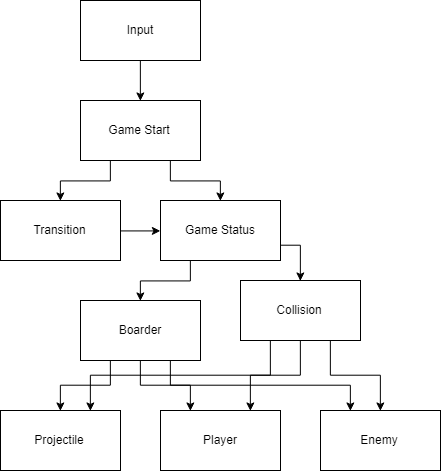
\includegraphics[width=0.7\textwidth]{Hierarchy.png}
\caption{Use hierarchy among modules}
\label{FigUH}
\end{figure}

%\section*{References}

\bibliographystyle {plainnat}
\bibliography {MG}

\end{document}